\documentclass[a4paper, 11pt]{article} % Font size (can be 10pt, 11pt or 12pt) and paper size (remove a4paper for US letter paper)

\usepackage[protrusion=true,expansion=true]{microtype} % Better typography
\usepackage{graphicx} % Required for including pictures
\usepackage{hyperref}
\usepackage{float}

\usepackage{mathpazo} % Use the Palatino font
\usepackage[T1]{fontenc} % Required for accented characters
\linespread{1.05} % Change line spacing here, Palatino benefits from a slight increase by default

\makeatletter
\renewcommand\@biblabel[1]{\textbf{#1.}} % Change the square brackets for each bibliography item from '[1]' to '1.'
\renewcommand{\@listI}{\itemsep=0pt} % Reduce the space between items in the itemize and enumerate environments and the bibliography

\renewcommand{\maketitle}{ % Customize the title - do not edit title and author name here, see the TITLE block below
\begin{flushright} % Right align
{\LARGE\@title} % Increase the font size of the title

\vspace{50pt} % Some vertical space between the title and author name

{\large\@author} % Author name
\\\@date % Date

\vspace{40pt} % Some vertical space between the author block and abstract
\end{flushright}
}

%----------------------------------------------------------------------------------------
%	TITLE
%----------------------------------------------------------------------------------------

\title{\textbf{Phylogeotool}\\ % Title
Installation Reference Manual} % Subtitle

\author{\textsc{Ewout Vanden Eynden, Pieter Libin, Kristof Theys, Guy Baele} % Author
\\{\textit{Rega Institute for Medical Research, KU Leuven}}} % Institution

\date{September 2016} % Date

%----------------------------------------------------------------------------------------

\begin{document}
\maketitle % Print the title section

\vspace{30pt} % Some vertical space between the abstract and first section

%------------------------------------------------
\tableofcontents
\newpage

\section{Installation}

\subsection{Using pre-built JAR files}
If you don't want to build the JARs/WAR from source, you can skip the following sections and proceed to section \ref{sec:jars}.

\subsection{Prerequisites for building your own}

\subsubsection*{Java}
Download and install the newest Java Development Kit (JDK) from \url{http://www.oracle.com/technetwork/java/javase/downloads/index.html}.
The current version of PhyloGeoTool was built using JDK 1.8.0\_31, but any Java version $>$7 should work.
For example, on Ubuntu Linux, Oracle Java 8 can be installed as follows (although OpenJDK should work just fine):
\begin{verbatim} 
sudo add-apt-repository ppa:webupd8team/java
sudo apt-get update
sudo apt-get install oracle-java8-installer
\end{verbatim}

\subsubsection*{Tomcat}
Download and install the latest Tomcat version from \url{http://tomcat.apache.org}.
For example:
\begin{verbatim}
sudo apt-get update
sudo apt-get install tomcat7
\end{verbatim}

\subsubsection*{Github}
Download the code from \url{https://github.com/rega-cev/phylogeotool/}. 
The project is currently still private. 
During the trial period you can send an email to \href{mailto:phylogeotool@kuleuven.be}  {phylogeotool@kuleuven.be} with your Github account name to get read rights on the project.
Git is readily available on most operating systems; if not, it can be installed as follows:
\begin{verbatim}
sudo apt-get install git-all
\end{verbatim}

\subsubsection*{Ant}
Download and install the newest Ant version from \url{http://ant.apache.org/} as we will use it to build our project.
The current version of PhyloGeoTool was built using Ant 1.9.4.
Ant can be installed as follows:
\begin{verbatim}
sudo apt-get install ant
\end{verbatim}

\subsubsection*{Phylogenetic tree}
A rooted binary phylogenetic tree in either Nexus or Newick format, which may or may not be time-stamped.

\subsubsection*{CSV file}
A comma-separated value (CSV) file, containing an ID column that contains IDs that correspond to the taxa names of the provided phylogenetic tree.
Remaining columns may contain additional information/annotation for the taxa in the phylogenetic tree, such as geographic location, virus genotype/subtype, patient attributes (age, ethnicity), \ldots \\
Information on the geography of taxa can be visualized in a map (Google Charts). For this to work, the column containing the geographic information needs to be configured with the "visualizeGeography" property in the XML configuration file (more information: section \ref{sssec:config_file}). The geographic values need to be formatted with the code or country name as defined in the ISO\_3166-1\_alpha-2 standard \footnote{\url{https://en.wikipedia.org/wiki/ISO\_3166-1\_alpha-2}}.  

\subsection{Building the project - Ubuntu Linux}

\subsubsection{Clone the git repository}
We here outline the various steps necessary for a successful build of the project.
The build process here is described as it was performed on an Ubuntu 14.04 LTS (Trusty Tahr) installation.
\begin{itemize}
\item Create an empty directory
\item {In that directory, clone the git repository: 
\begin{verbatim}
git clone https://github.com/rega-cev/phylogeotool/
cd phylogeotool
ant
\end{verbatim}
\item This build process generates a phylogeotool-01.war, DistanceMatrix.jar and PreRender.jar in the dist directory.
}
\end{itemize}


\subsubsection{DistanceMatrix.jar}
\label{sec:dm}
This jar file contains a tool to create a distance matrix, which will be used in the next section, based on the phylogenetic tree that will be used in the PhyloGeoTool.
DistanceMatrix.jar uses one input file, a phylogenetic tree to be used in the PhyloGeoTool, and will output the distance matrix that is derived from the phylogenetic tree.
For example, the following command uses DistanceMatrix.jar to generate a distance matrix (to be stored in a file called distances.csv in the command below) from a previously reconstructed phylogenetic tree in Newick format: 
\begin{verbatim}
java -jar DistanceMatrix.jar tree.newick distances.csv
\end{verbatim}


\subsubsection{PreRender.jar}
A major goal of the PhyloGeoTool is to cluster the tree index the taxa annotations, of which the computation takes a long time and its runtime depends on the size of the phylogenetic tree. 
However, this computation can be performed before the installation of the web-tool, using PreRender.jar and making use of the DistanceMatrix.jar, allowing the web-tool to render both clusters and annotations instantaneously.

PreRender.jar takes the following arguments: 
\begin{itemize}
\item /path/to/phylogenetic.tree: Link to the phylogenetic tree used in the PhyloGeoTool.
\item /path/to/csvFile: Link to the csv file that connects nodes in the tool to attributes. Note: The id in the csv file has to be the same as the id of the nodes in the tree.
\item /path/to/distance\_matrix: Link to the distance matrix (see section \ref{sec:dm}) that was generated from this tree.
\item /path/to/folder\_output: Link to the folder where this jar can write its resulting tree files.
\item /path/to/rBinary: Link to the exact location of the executable to run R 
\item /path/to/folder\_rScripts: Link to the folder which contain SDR.R, FirstDerivative.R, sgolay.R and SecondDerivative.R
\end{itemize}
PreRender.jar will then create the necessary directories in the folder with name `folder\_output'.
If those directories already exist, a warning is issued to the user and the process will be aborted.

For example, the following command uses PreRender.jar to perform all the necessary clustering steps (which can be time-consuming) so that the PhyloGeoTool doesn't have to perform these at run time: 
\begin{verbatim}
java -jar PreRender.jar phylogenetic.tree csvFile
distance\_matrix folder\_output rBinary folder\_rScripts
\end{verbatim}


\subsubsection{Create a config file} \label{sssec:config_file}

In the /etc folder, create a directory `phylogeotool', which is the default location for the config file:
\begin{verbatim}
sudo mkdir phylogeotool
cd phylogeotool
touch global-conf.xml
\end{verbatim}

An example of such a configuration file can be found here: \url{https://github.com/rega-cev/phylogeotool/blob/master/examples/global-conf.xml}.
In the XML file, we assume a user name 'phylogeo' to perform the installation.

%GB: Ewout, can you replace the XML code below by the latest version of such a global-conf.xml file?
Edit the global-conf.xml file to correctly set up all the necessary paths, example content of global-conf.xml is shown here (assuming that all the data resides in subfolders of /Users/phylogeo/Documents/):
\begin{verbatim}
<?xml version="1.0" encoding="UTF-8"?>
<phylogeotool-settings>
  <!-- basePath
     Root directory containing the pre-rendered files in 
     subdirectories such as given to PreRender.jar.
   -->
  <property name="basePath">
    /Users/phylogeo/Documents/Configs
  </property>

  <!-- metadataFile
   Pointer to the location of the csv file containing all the 
   information on the individual sequences.
  -->
  <property name="metadataFile">
   /Users/phylogeo/Documents/Configs/metadataFile.csv
  </property>

  <!-- phyloTreeFile
   Pointer to the location of the phylogenetic tree file.
  -->
  <property name="phyloTreeFile">
   /Users/phylogeo/Documents/Configs/phylo.tree
  </property>

  <!-- alignmentFile
   Pointer to the location of the alignment file that was used 
   to build the phylogenetic tree used in this tool.
   This is only needed in case the user of PPlacer 
   should be supported in the tool.
  -->
  <property name="alignmentFile">
    /Users/phylogeo/Documents/Configs/alignment.fasta
  </property>
  
  <!-- logFile
   Pointer to the logfile file that was returned by the tree 
   building program to build the phylogenetic tree used in this 
   tool, as for example generated by FastTree if specified 
   as an option (RAxML and PhyML generate it by default).
   This file is only needed in case PPlacer should be 
   supported in the tool.
  -->
  <property name="logFile">
    /Users/phylogeo/Documents/Configs/logFile.log
  </property>

  <!-- scriptFolder
   Pointer to the location of the shell scripts that are 
   used to initiate PPlacer.
   This folder should contain fasta_subsample.pl, init.sh 
   and place.sh, which can be found here:
   https://github.com/rega-cev/phylogeotool/blob/master/scripts/
  -->
  <property name="scriptFolder">
    /Users/phylogeo/Documents/PPlacer
  </property>

  <!-- showNAData 
   Include Non Assigned (NA) data in the graphs
  -->
  <property name="showNAData">
    false
  </property>
  
  <!-- visualizeGeography 
   Fill in the field that has to be visualized on the map in the tool.
  -->
  <property name="visualizeGeography">
  	COUNTRY_OF_ORIGIN_EN
  </property>

  <!-- 
   Color codes used for the google chart
  -->
  <property name="colorCodes">
    <chart name="datalessregion">#FFFFFF</chart>
    <chart name="backgroundcolor">#FFFFFF</chart>    
    <chart name="colorAxis">#e9e9e9,red</chart>
  </property>
  
  <!-- PPlacer Support
  Indication if PPlacer should be supported in the PhyloGeoTool
 -->
 <property name="pplacer_support">
 true
 </property>

 <!--
   How the csv field should be represented in the tool.
   A number field will be shown in a histogram
   A string field will be shown as a category chart
 -->
 <property name="csvFieldRepresentation">
   <dataField name="header1" type="number">PATIENT_ID</dataField>
   <dataField name="header2" type="string">GENDER</dataField>
 </property>
</phylogeotool-settings>
\end{verbatim}



\subsubsection{Start Tomcat server and load phylogeotool}

Copy the phylogeotool-01.war to the webapps folder of Tomcat and start Tomcat:
\begin{verbatim}
sudo cp phylogeotool-01.war /var/lib/tomcat7/webapps/
cd /var/lib/tomcat7/
sudo service tomcat7 restart
\end{verbatim}
This enables browser access to a localhost version of the PhyloGeoTool.
Open a browser and enter the following URL: \url{http://localhost:8080/phylogeotool/PhyloGeoTool}.
The browser should show something similar to Figure \ref{fig:01}.


\begin{figure}[!htbp]
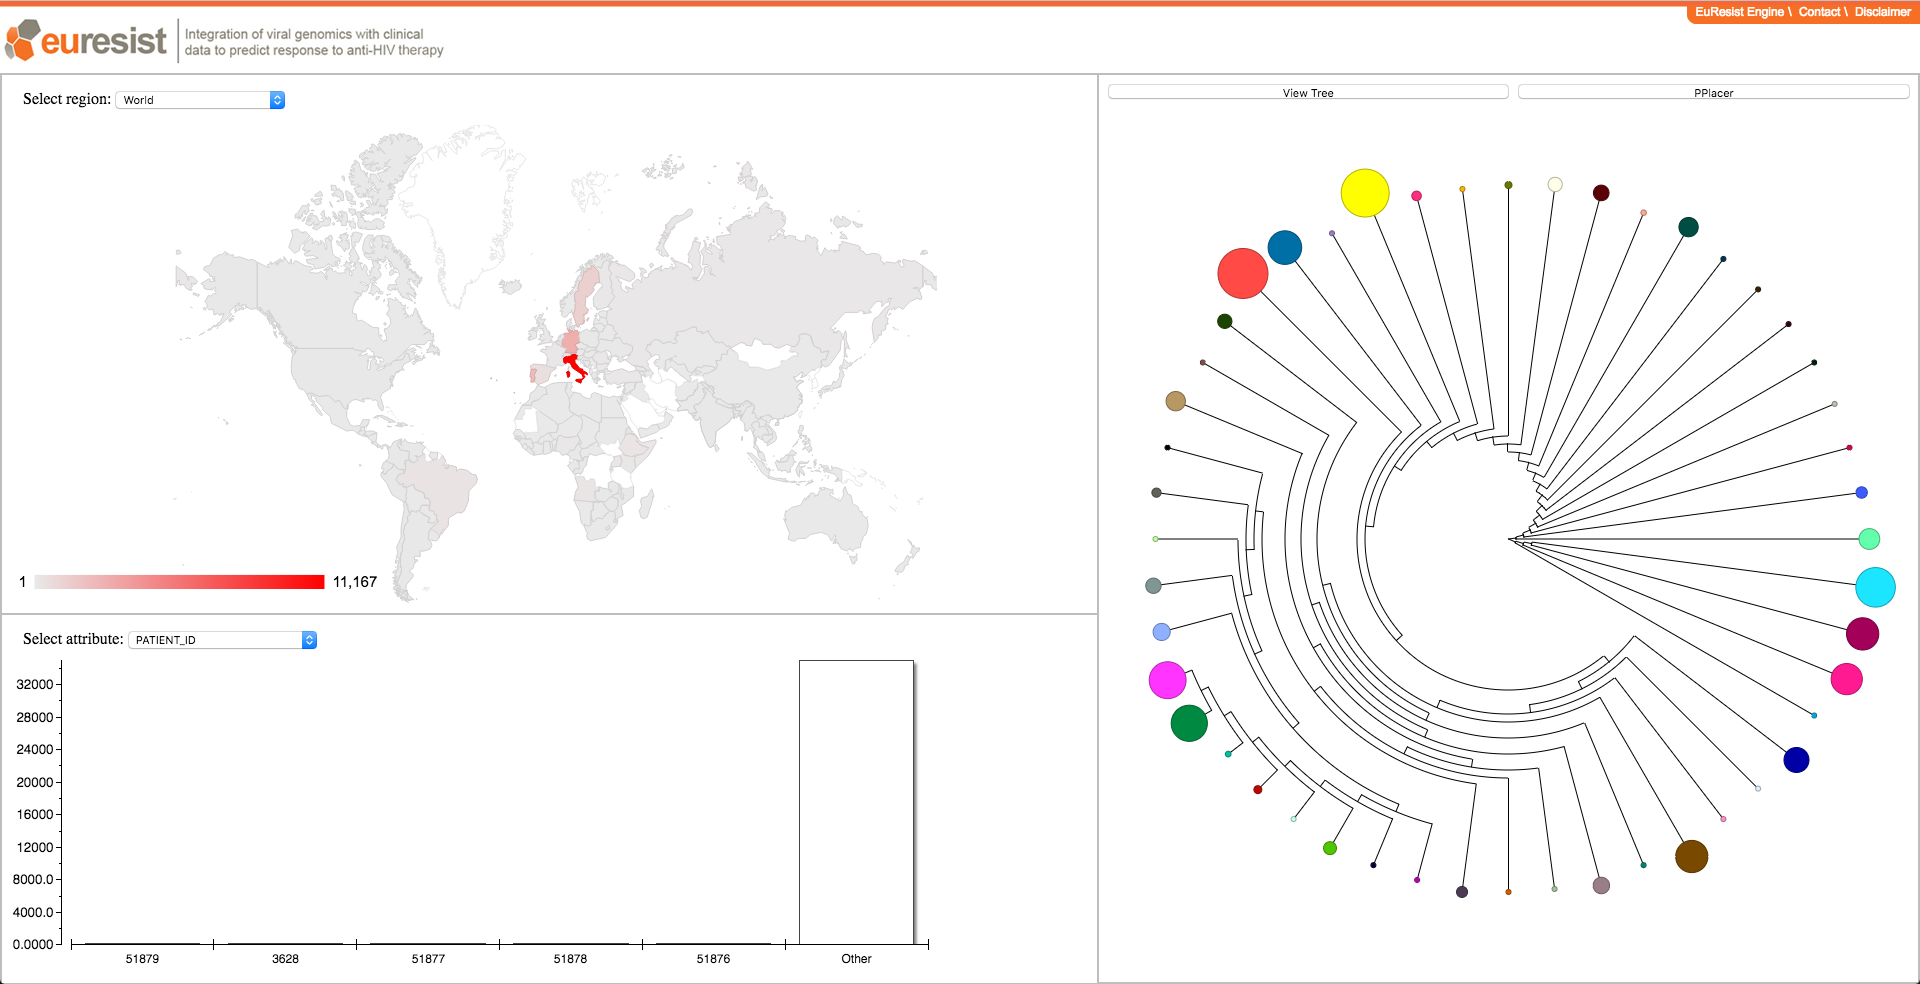
\includegraphics[scale=0.19]{images/defaultScreenshot.png}
\caption{Screenshot of the PhyloGeoTool application when the application is started for the first time.}
\label{fig:01} 
\end{figure}





\end{document}
